\section{Image Filtering}
\greenbf{Operator *} mapping image and kernel to images: $I_out = k * I_in$\\
\greenbf{Local:}$I_{out}[i, j]$ depends only on neighbors of $I_{in}[i,j]$\\
\greenbf{Associative:} $((k_1 * k_2) * I) = (k_1 * (k_2 * I))$\\
\greenbf{Shift invariant:} $shift(k * I) = k * shift(I)$\\
\greenbf{Linear:} $k * (\alpha I_1 + \beta I_2) = \alpha (k * I_1) + \beta (k * I_2)$\\
\greenbf{Linear Combination of neighbors:} \\
$\sum_{\begin{subarray}{c}
    (i, j) \in \underbrace{\mathbb{N}(x, y)}_{\text{neighborhood}}
\end{subarray}}
K(x, y, i, j) \underbrace{I}_{\text{Input}} (x + i, y + j)$

\greenbf{Filter at edges:} clip filter (black), wrap around, copy edge, reflect across edge, vary filter near edge
\subsection*{Correlation}
$I'(x, y) = \sum_{(i, j) \in \N(x, y)} K(i, j) I (x + i, y + j)$ \\
$I' = K \circ I \quad$ e.g. template matching: search for best match by minimizing mean squared error or maximizing area correlation. (remove mean (from filter, from image) to avoid bias)
\subsection*{Convolution}
$I' = K * I, I'(x, y) = \sum_{(i, j) \in \N(i, j)} K(i, j) I (x - i, y - j)$ if $K(i, j) = K (-i, -j) \implies \\
correlation = convolution \quad\\
convoution = correlation + \text{ filter rotated 180°}$\\
\greenbf{Continuous:} $(f * g)(t) \\
= \int_{-\infty}^{\infty} f(\tilde{t}) g(t - \tilde{t}) d\tilde{t}\\
= \int_{-\infty}^{\infty} f(t - \tilde{t}) g(\tilde{t}) dt$
\subsection*{Kernels}
\greenbf{separable:} if a kernel can be written as a product of two simpler filters $\rightarrow$ computationally faster (filter $P \times Q$, image $N \times M: (P + Q) * NM$ instead of $PQNM$)\\
Separable filters can be written as \( K(m,n) = f(m)g(n) \).
For a rectangular neighborhood with size \((2M+1) \times (2N+1), I'(m, n) = \fcolorbox{green}{white}{f * (\fcolorbox{red}{white}{g * I(N(m, n))})}\)\\
$
\fcolorbox{red}{white}{I''(m,n)} = \sum_{j=-N}^{N} g(j) I(m, n - j)
$
\\
$\fcolorbox{green}{white}{I'(m, n)} = \sum_{j=-N}^{N} f(i) I''(m - i, n)$\\
\greenbf{Box filter:} all same values normalized to sum = 1\\
\greenbf{Gaussian Kernel:} $K(x, y) = \frac{1}{2\pi \sigma^{2}} e^{-\frac{x^{2} + y^{2}}{2\sigma^{2}}}$ is separable, e.q. $\sigma = 1$\\
Gaussian Smoothing Kernel Top-5
\begin{compactitem}
\item Rotationally symmetric
\item has single lobe \graytext{Neighbor's influence decreases monotonically}
\item Still one lobe in frequency domain ,\graytext{No corruption from high frequencies}
\item Simple relationship to $\sigma$
\item Easy to implement efficiently
\end{compactitem}
\greenbf{High Pass Filter:}
high pass filter detects edges 
High Pass Filter Laplacian Operator \\
$
\begin{bmatrix}
   % \begin{smallmatrix}
        -1 & -1 & -1 \\
        -1 & 8 & -1 \\
        -1 & -1 & -1 \\
    %\end{smallmatrix}
\end{bmatrix} 
$$
\begin{bmatrix}
    %\begin{smallmatrix}
        0 & 1 & 0 \\
        1 & -4 & 1 \\
        0 & 1 & 0 \\
    %\end{smallmatrix}
\end{bmatrix} 
$
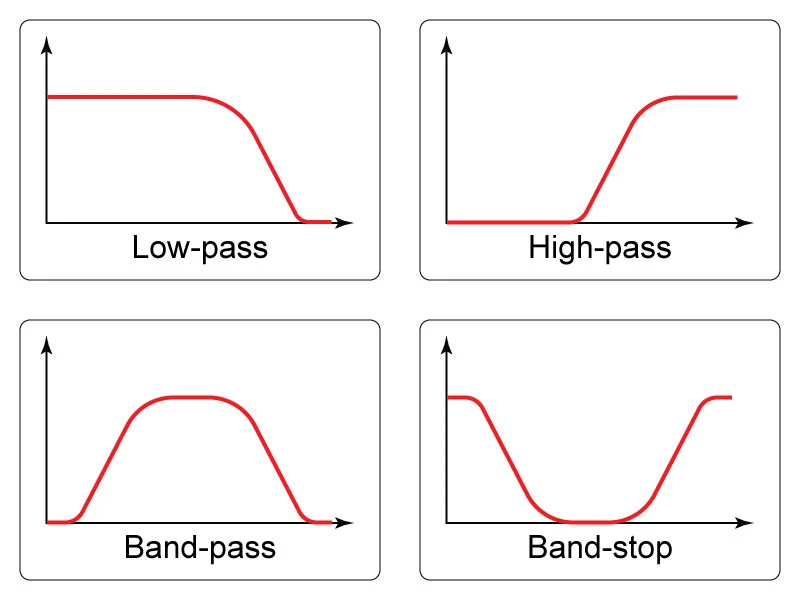
\includegraphics[width = 0.3 \columnwidth]{assets/jo/Types_of_Filters.png}

\greenbf{Low Pass Filter:}
blurs (detects "smooth" regions) Gaussian Filter is a low pass filter, proof: Convolution theorem: Fourier transform H of h is equal to $F \cdot G$
If $g$ is Gaussian, its Fourier Transform $G$ is also Gaussian.
Pointwise multiplication of $F$ with $G$ will keep the low frequencies of F unchanged, while the high frequencies will be multiplied by a low number, and therefore, they will be removed.  \\
\greenbf{Conversion:} Subtracting one from central element of low-pass filter gives a high-pass filter with inverted sign, because.\\
$(f - \delta) * a = f * a - \delta * a = f * a - a = - (a - (f * a))$ Normalize the low-pass kernel and then subtract one from central element. Normalize low-pass filter, then subtract the kernel from central element matrix. To get the high pass filter, you do not need to normalize.\\
\greenbf{Band pass filter:} 
\includegraphics*[width = 0.4cm]{jo/band-pass-filter.png}
do LPF and HPF with cutoffs $f_{LP} < f_{HP} \quad f = \text{ cut of frequencies, cannot coincide}$\\
Filter image with high-pass and low-pass filter to get band pass filter. \graytext{Only works when you have an overlap in frequencies. If no overlap: $I *_{convolution} (\delta - f_{LP - f_{HP}}) \rightarrow $ gap between is band filter.}\\
\greenbf{Band reject filter:} \includegraphics*[width = 0.4cm]{jo/band-reject-filter.png}
do LPF and HPF with cutoffs $f_{LP} > f_{HP}$\\
\greenbf{Image sharpening:} increases high frequency components to enhance edges: $I' = I + \alpha |K * I|$ $K:$ high-pass filter, $\alpha$: scalar $\in [0, 1]$